\documentclass[conference]{IEEEtran}
\RequirePackage{cite}
\RequirePackage{amsmath,amssymb,amsfonts}
\RequirePackage{algorithmic}
\RequirePackage{graphicx}
\RequirePackage{textcomp}
\RequirePackage{xcolor}
\RequirePackage{hyperref}
\RequirePackage{csquotes}
\setkeys{Gin}{width=0.4\textwidth}
\def\BibTeX{{\rm B\kern-.05em{\sc i\kern-.025em b}\kern-.08em
    T\kern-.1667em\lower.7ex\hbox{E}\kern-.125emX}}
\begin{document}
\title{EECS 106B Final Project Proposal}
\author{Andrew~Fearing, Neelay~Junnarkar,  Hamza~Kamran~Khawaja}
\maketitle


\begin{abstract}
We want to get a sailboat (a type of Unmanned Surface Vehicle, or USV) through a canal autonomously. The maneuver will be performed in a simulation environment such as Matlab/Simulink, with simulated wind as the propellant for the USV. Environmental disturbances (water currents) will also be an important factor. We will utilize a Control Barrier Function, building upon foundational work in \cite{Ames2017} and \cite{Ames2019} with a feedback controller to create a robust control scheme for navigation through the canal.

\end{abstract}


\section{About Us}
Neelay is a 4th year undergraduate in EECS, and has taken courses such as EE 128, 221A/222, and (of course) EECS 106A. His interests are primarily related to control and motion planning.

Andrew is a 4th year undergraduate in EECS. He has taken EE 120, EE C128, and EECS C106A. His interests in robotics are in micro-scale mobile robots.

Hamza is a 4th year undergraduate in EECS. He has taken EECS106A,and EECS126. His interests in robotics are in machine learning/ artificial intelligence and dynamically responsive, maneuverable robotic systems with a spice of efficiency/optimization.

\section{Research Question}
Can we control a sailboat so that it safely navigates a channel, even with environmental disturbances such as wind and waves? How much disturbance can we make the sailboat robust to?
Some problems facing steering a sailboat in a confined space include perturbations such as wind gusts and waves. Further, some techniques such as tacking, used when sailing into the wind, inherently use side-to-side motion.

\section{Motivation}
 Existing systems to survey and navigate the ocean surface include fixed monitoring systems, that either drift (floating buoys) or are fixed (moored data-buoys), survey ships and satellites. The floating buoys are easily lost, the moored buoys are expensive to deploy and maintain, survey ships are limited in range, and satellites take a long time to manufacture with high cost and lack the resolution and accuracy of in-situ devices \cite{Sauze2006}.
\begin{figure}
    \centering
    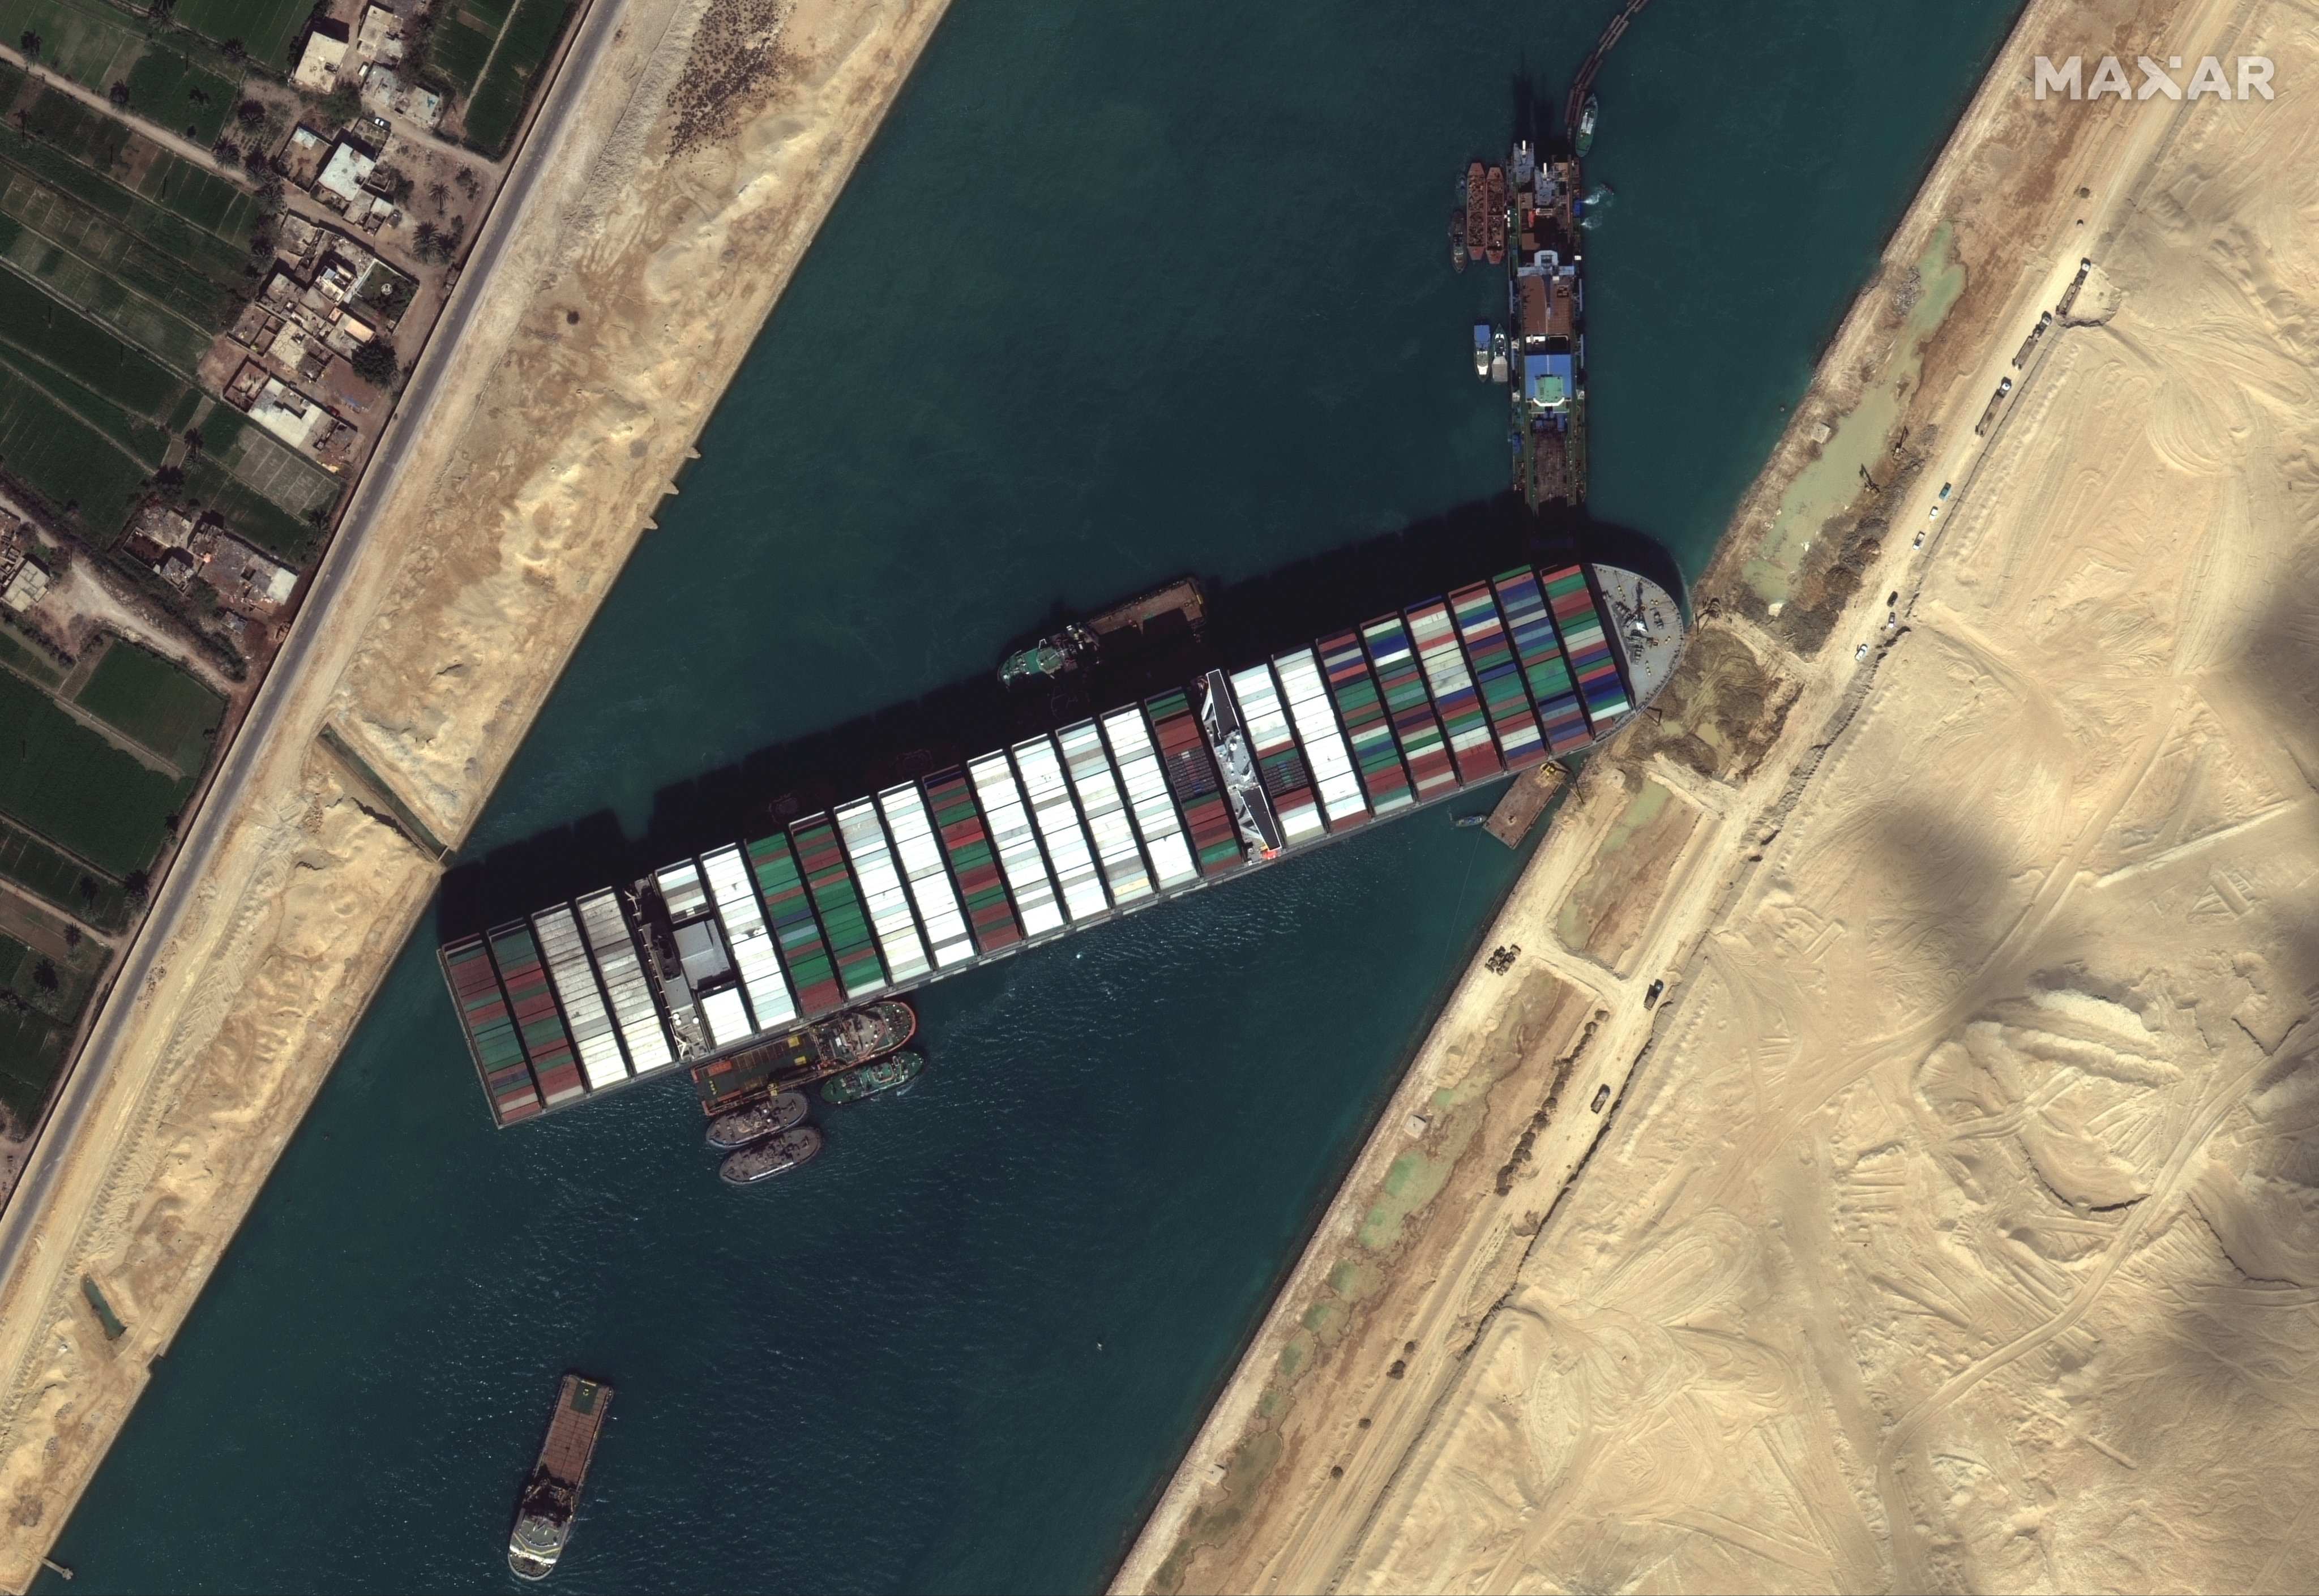
\includegraphics{documents/proposal/Suez_Canal_blocked_by_Ever_Given_March_27_2021.jpg}
    \caption{Boat stuck (what we want to avoid)\label{fig:boat_stuck}}
\end{figure}
Control and safety of automobiles is an area of intense research focus. We want to try applying similar techniques to a different system: autonomous boats, or in engineering terms, \enquote{Unmanned Surface Vehicles} (USV). In particular, we will be looking at autonomous sailboats, since our literature review shows there has been less work on sailboats than on motorboats.
Sailboats are able to operate with little power requirements, instead leveraging energy from the wind, lending themselves to long-term autonomous operation.

\section{Proposed Methodology}
We plan to use simulation to quantify the performance of our control scheme. We will examine literature in USV's.
We will simulate an autonomous sailboat with realistic environmental disturbances.
Then we will maneuver the sailboat through a canal passage, propelled purely with wind energy. Ranges and limitations will be observed and path-planning/boat dynamics will allow us to navigate the autonomous sail-boat without capsizing and without collision with the canal boundaries. 

We will need to carefully define the scope of our project. At the moment, it is not clear how high the fidelity of our simulation will need to be.
\section{Related Work}
USV's have been an area of research since at least WWII. In the 1990's, the field expanded, focusing on control and navigation for motorboats. More recently in the 2010's and 2020's, more research has come out that focuses on autonomous sailboats.




\cite{Setiawan2020} and \cite{Buehler2018} develop dynamic models of an autonomous sailboats, though they do not go into the application of controls. These dynamical models will be useful to abstract the sailboat system (in particular from all the physics), so we can develop controllers off of these.

\cite{Xiao2014} studies nonlinear heading control of a 4-DOF autonomous sailboat model, taking into account wind but no water disturbances. This paper may be a useful resource since we are attempting to study an extension of this problem.

\cite{Velueta2019} develops sliding mode control techniques for motorboats, focusing on robustness with respect to water waves. These papers show control schemes on related models, and will be useful references while we develop controllers on sailboat dynamical models.

We hope to incorporate the control barrier functions we learned about in our presentation on \cite{Ames2019} to provide robustness. In \cite{Ames2017}, methods to use control barrier functions for autonomous car lane keeping are presented, which may be useful to develop a parallel methodology for the sailboat dynamical model.

\section{Experimental Plan}
Using a dynamic model as that proposed in \cite{Buehler2018}, we will simulate and analyze the performance of our control scheme. We will simulate an autonomous sailboat with realistic environmental disturbances using a simulation environment e.g Matlab/Simulink, Gazebo, VREP, or USVSim. Our decision for the fidelity and resolution will determine which of these environments would perform best. One factor that we will need to decide is whether we need both wind and water wave simulation, or just wind simulation. Simulated wind from the environment will be the only source of propulsion. Our sailboat model will have two actuators: a sail and a rudder. Our control scheme will be similar to that of \cite{HelmiAbrougui2019}, shown in Fig.~\ref{fig:control_scheme.png}

\begin{figure}
    \centering
    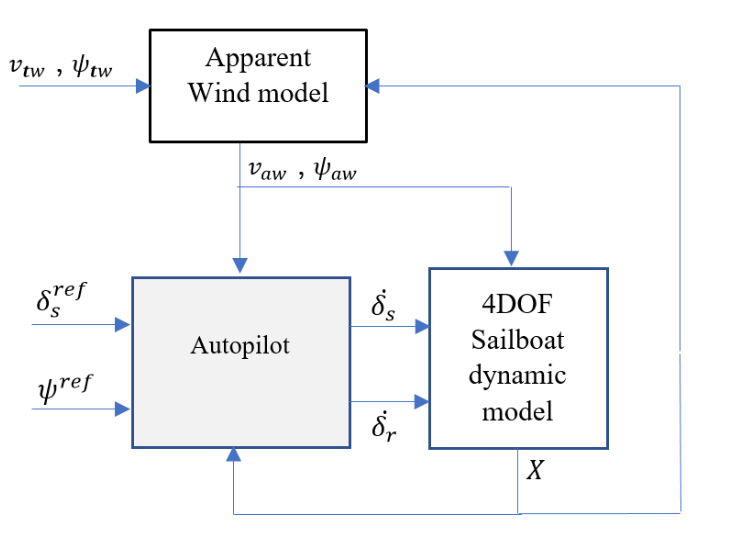
\includegraphics{documents/proposal/control_scheme.PNG}
    \caption{Control scheme with inputs and outputs from \cite{HelmiAbrougui2019}}
    \label{fig:control_scheme.png}
\end{figure}


\bibliographystyle{IEEEtran}
\bibliography{refs.bib}
\end{document}